
%(BEGIN_QUESTION)
% Copyright 2007, Tony R. Kuphaldt, released under the Creative Commons Attribution License (v 1.0)
% This means you may do almost anything with this work of mine, so long as you give me proper credit

The following binary logic diagram shows a two-out-of-three detector scheme for a flame safety system:

$$\includegraphics[width=15.5cm]{i02331x01.eps}$$

The purpose of this logic system is to indicate whether or not at least {\it two} flame detectors are showing the presence of flame in a burner system.  Here, flame is good, and no flame is bad.  Explain how this logic system works, and relate the symbols contained within to traditional logic symbols such as these shown below:

$$
\includegraphics[width=15.5cm]{i02331x02.eps}$$

\underbar{file i02331}
%(END_QUESTION)





%(BEGIN_ANSWER)

Other than the AND and OR symbols looking a bit different, there is little else in the binary logic diagram that should cause confusion to someone already familiar with the rounded logic gate symbols.

\vskip 10pt

Follow-up question: what do you think might be suggested by the oval bubbles versus the pointed box, showing inputs and outputs in this diagram, respectively?  I'll give you a hint: the different shapes do {\it not} simply spell the difference between input and output!

%(END_ANSWER)





%(BEGIN_NOTES)

Note how the oval bubbles lie within the ``field'' area, meaning they are inputs coming from actual field devices.  The pointed box lies inside the logic area, making it an internal variable to that system.

\vskip 10pt

The form of logic diagram shown in the question is often standard in distributed control systems (DCS) and other computer-based logic controls.  It is based on the 2002 revision of ISA's S5.2 standard, now ANSI/ISA-5.01.01.  The original ISA S5.2 standard is similar, with some minor differences.  

Discuss with your students what all the symbols mean, and how they relate to electronic logic schematics with more traditional AND, OR, and NOT gate symbols.

%INDEX% Documentation, binary logic: two-out-of-three logic (2oo3)

%(END_NOTES)


